%%%%%%%%%%%%%%%%%%%%%%%%%%%%%%%%%%%%%%%%%
% Beamer Presentation
% LaTeX Template
% Version 1.0 (10/11/12)
%
% This template has been downloaded from:
% http://www.LaTeXTemplates.com
%
% License:
% CC BY-NC-SA 3.0 (http://creativecommons.org/licenses/by-nc-sa/3.0/)
%
%%%%%%%%%%%%%%%%%%%%%%%%%%%%%%%%%%%%%%%%%

%----------------------------------------------------------------------------------------
%	PACKAGES AND THEMES
%----------------------------------------------------------------------------------------
%!TEX encoding = UTF-8 Unicode


\documentclass[12pt,handout]{beamer}
\usepackage[utf8]{inputenc}
\usepackage{amsmath}
\usepackage[T1]{fontenc}
\usepackage{verbatim}

\mode<presentation> {

\usetheme{Pittsburgh}

}

\usepackage{graphicx} % Allows including images
\usepackage{booktabs} % Allows the use of \toprule, \midrule and \bottomrule in tables

%----------------------------------------------------------------------------------------
%	TITLE PAGE
%----------------------------------------------------------------------------------------

\title[]{Critical behaviour of the surface tension in the 3D Ising model} % The short title appears at the bottom of every slide, the full title is only on the title page

\author[]
{
Federico Belliardo \\
Marco Costa
} 

\institute[] % Your institution as it will appear on the bottom of every slide, may be shorthand to save space
{
Dipartimento di Fisica\\ % Your institution for the title page
Università di Pisa \\
\medskip
}
\date{\today} % Date, can be changed to a custom date

\begin{document}

\begin{frame}
\titlepage % Print the title page as the first slide
\end{frame}

%\begin{frame}
%\frametitle{Overview} % Table of contents slide, comment this block out to remove it
%\quadleofcontents % Throughout your presentation, if you choose to use \section{} and \subsection{} commands, these will automatically be printed on this slide as an overview of your presentation
%\end{frame}

%----------------------------------------------------------------------------------------
%	PRESENTATION SLIDES
%----------------------------------------------------------------------------------------

\begin{frame}{Summary}

\begin{center}

\begin{itemize}
\item 3D Ising models
\item Definition of the surface tension
\item Cluster algorithms and boundary flip
\item (Notes on the implementation?)
\item Estimation of the errors and autocorrelation
\item Fit of the free energy
\item Fit of the critical behaviour
\item (Conclusion?)
\end{itemize}

\end{center}
\end{frame}

\begin{frame}{3D Ising model}
\begin{center}
\begin{columns}
\begin{column}{0.43\textwidth}
 \[
\mathcal{H} = -\sum_{\langle x, y \rangle} J_{\langle x, y \rangle} s_x s_y
\]

\[
J_{\langle x, y \rangle} = 1\text{ ferromagnetic}
\]
\[
J_{\langle x, y \rangle} = -1\text{ antiferromagnetic}
\]
\end{column}

\begin{column}{0.57\textwidth}  %%<--- here
 \begin{figure}[!htb]
\centering
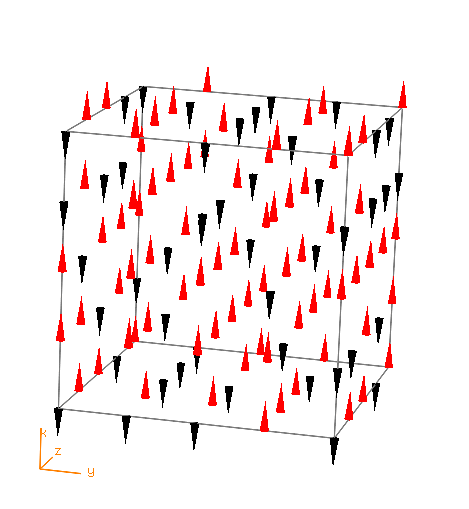
\includegraphics[scale=0.5]{ising3D.png}
\end{figure}
\end{column}
\end{columns}


\end{center}
\end{frame}

\begin{frame}{Definition of the surface tension}
\begin{center}


\begin{figure}[!htb]
\centering
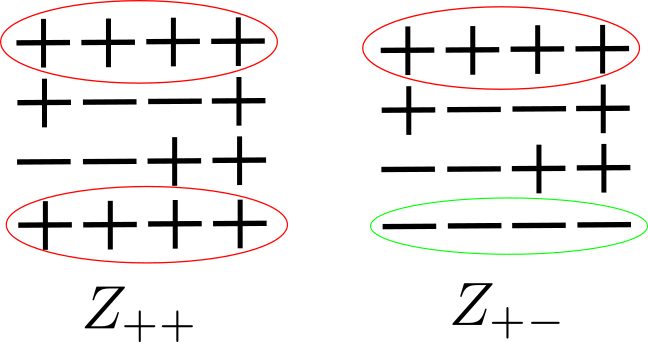
\includegraphics[scale=0.5]{bound.png}
\end{figure}

\vspace{20pt}

{\Large
$
\sigma = -\lim_{L \rightarrow \infty} \frac{1}{L^2} \log \frac{Z_{+-}}{Z_{++}}$} $ \quad L \times L \times T,\, T = cL$

\note{L'ordine dei due limiti T e  non dovrebbe contare. Non so se si può "dimostrare" al nostro libello di rigore fisiamo T = 3L e facciamo il limite per L. Per sistemare la faccenda introduciamo una larghezza L del sistema e questa è l'unica lunghezza che va all'infinito.}

\note{$Z_{+-}$ e $Z_{++}$ sono le funzioni di partzione quando fisso cosa devono valere i layer di spin sul pavimento e sul soffito. Inserire piccola immagine per spiegarlo.}

\end{center}
\end{frame}

\begin{frame}
\begin{center}
\begin{figure}[!htb]
\centering
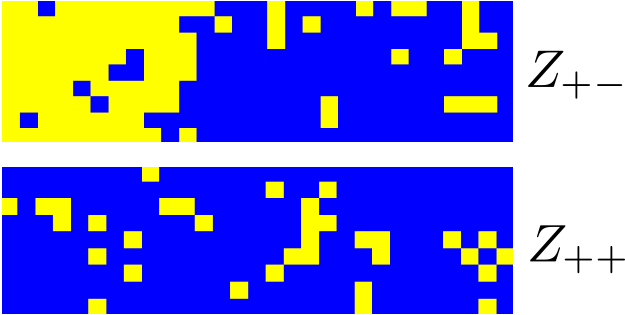
\includegraphics[scale=0.50]{comparison.png}
\end{figure}
\[
\sigma = -\lim_{L \rightarrow \infty} \frac{1}{L^2} \log \frac{Z_{+-}}{Z_{++}} = \lim_{L \rightarrow \infty} \frac{1}{L^2} \left( F_{+-} - F_{++} \right) = \lim_{L \rightarrow \infty} \frac{F_s}{L^2}
\]
\[\sigma = \text{interface free energy per unit area}\]

\note{Bisogna dire che nel limite termodinamico sopravvive una sola superficie di separazione.}

\end{center}
\end{frame}

\begin{frame}
\begin{center}

\begin{columns}
\begin{column}{0.50\textwidth}
\begin{center}
Redefinition of $Z_{++}$ and $Z_{+-}$.\\
\vspace{10pt}
$Z_{++} \rightarrow $ ferromagnetic link between \textbf{top and bottom}.\\
$Z_{+-} \rightarrow $ \textbf{anti}ferromagnetic link between \textbf{top and bottom}.\\
\vspace{10pt}
Always ferromagnetic link in $x$ and $y$.\\
\vspace{10pt}
Same definition for $\sigma$.\\
\vspace{10pt}
Periodic boundary conditions reduce the finite size effect.\\
\end{center}

\end{column}
\begin{column}{0.50\textwidth}

\begin{figure}[!htb]
\centering
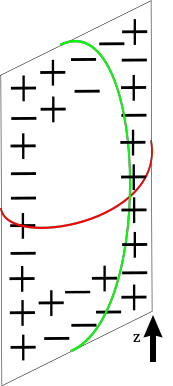
\includegraphics[scale=0.7]{antiferro.png}
\end{figure}

\end{column}
\end{columns}

\end{center}
\end{frame}

\begin{frame}
\begin{center}
{\Large Montecarlo simulations can't measure $Z$!\\}
\vspace{10pt}
Solution: $J_{\langle x, y \rangle}$ between top and bottom becomes a \textbf{dinamical variable} that is summed over in $Z$.\\
$J_{\langle x, y \rangle} = 1$ (periodic b.c.)\hspace{10pt}$J_{\langle x, y \rangle} = -1$ (antiperiodic b.c.)\\
Other $J_{\langle x, y \rangle}$ remains ferromagnetic.

\[
Z = \sum_{\lbrace s \rbrace, J} \exp \left( \beta \sum_{\langle x, y \rangle} J_{\langle x, y \rangle} s_x s_y \right)
\]

{\large \[
\frac{Z_{+-}}{Z_{++}} = \frac{\frac{Z_{+-}}{Z}}{\frac{Z_{++}}{Z}}=\frac{\langle \delta_{J = -1} \rangle}{\langle \delta_{J = + 1} \rangle}
\]}

Ratio of measurable expectation values.
\end{center}
\end{frame}

\begin{frame}
\begin{center}
We redefine the free energy of the interface in order to improve the convergence proprieties of $\frac{F_s}{L^2}$ to $\sigma$ when $L \rightarrow \infty$.
\vspace{10pt}
Thermodynamic limit {\Large $\rightarrow$} only \textbf{one} interface\\
\vspace{10pt}
For finite $L$ multiple interface can be present. An even number for $Z_{++}$ and odd for $Z_{+-}$.\\

\begin{figure}[!htb]
\centering
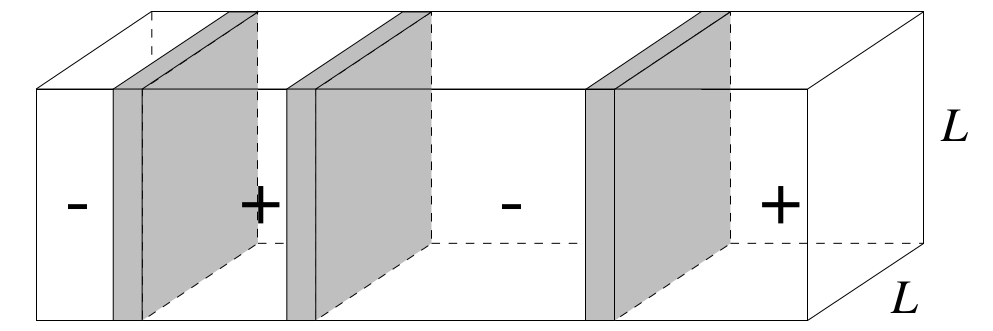
\includegraphics[scale=0.3]{multiple.png}
\end{figure}

\end{center}
\end{frame}

\begin{frame}
\begin{center}

$F_s$ is the free energy of a single surface. There are $\sim T$ different position for the interface.
\[Z_1 = T \exp \left( - F_s \right) = \exp \left( -F_S +\ln T \right) \]

\[ \frac{Z_{+-}}{Z_{++}} = \frac{Z_1 + \frac{Z_1^3}{3!} + \frac{Z_1^3}{5!} + ...}{1 +  \frac{Z_1^2}{2!} + \frac{Z_1^4}{4!} + ...} = \tanh \left( \exp \left( -F_S +\ln T \right) \right) \]

\[
F_S = \ln \left( T \right) - \ln \left( \frac{1}{2} \ln \left( \frac{1 + \frac{Z_{+-}}{Z_{++}}}{1 - \frac{Z_{+-}}{Z_{++}}} \right) \right) \quad \sigma = \lim_{L \rightarrow \infty} \frac{F_s}{L^2} \]


\end{center}
\end{frame}

\begin{frame}{Cluster algorithms and boundary flip}
\begin{center}

Cluster algorithms allow for simultaneous updates of large parts of the lattice. Thus reducing the autocorrelation time and the critical slowling down. Swendsen and Wang (1987).\\
\vspace{10pt}
Introduce link variables $\sigma_{\langle x, y \rangle} = \lbrace 0, 1 \rbrace$ on the lattice:

\begin{figure}[!htb]
\centering
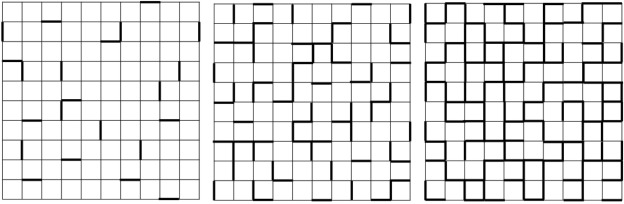
\includegraphics[scale=0.4]{link.png}
\end{figure}

\note{Giustificare perché metto tre reticoli. Sono a diversa temperatura. A bassa T (alto beta) è facile formare i cluster. A basso beta è difficile.}

\end{center}
\end{frame}

\begin{frame}
\begin{center}

\begin{gather*}
Z = \sum_{\lbrace s = \pm 1\rbrace} \exp \left( \beta \sum_{\langle x, y \rangle} s_x s_y \right) = \sum_{\lbrace s = \pm 1 \rbrace} \prod_{\langle x, y \rangle} e^{ \beta  s_x s_y} = \\[20pt]
= e ^{ -d V \beta } \sum_{\lbrace s = \pm 1 \rbrace} \prod_{\langle x, y \rangle} \left( 1 + \delta_{s_x, s_y} \left( e^{  2 \beta} - 1 \right) \right) = \\[20pt]
= e^{ -d V \beta} \sum_{\lbrace s \rbrace} \prod_{\langle x, y \rangle}   \sum_{\lbrace \sigma_{\langle x, y \rangle} = 0,1 \rbrace} \left[ \left( 1 - \sigma_{\langle x, y \rangle} \right)
+ \sigma_{\langle x, y \rangle} \delta_{s_x, s_y} \left( e^{ 2 \beta } - 1 \right) \right]
\end{gather*}

\end{center}
\end{frame}

\begin{frame}
\begin{center}

Also valid for generic coupling $J_{\langle x, y \rangle}$:

\begin{gather*}
Z = \sum_{\lbrace s = \pm 1\rbrace} \exp \left( \beta \sum_{\langle x, y \rangle} J_{\langle x, y \rangle} s_x s_y \right) = \sum_{\lbrace s = \pm 1 \rbrace} \prod_{\langle x, y \rangle} e^{ \beta  J_{\langle x, y \rangle} s_x s_y} = \\[20pt]
= e ^{ -d V \beta } \sum_{\lbrace s = \pm 1 \rbrace} \prod_{\langle x, y \rangle} \left( 1 + \delta_{J_{\langle x, y \rangle} s_x s_y, 1} \left( e^{  2 \beta} - 1 \right) \right) = \\[20pt]
= e^{ -d V \beta} \sum_{\lbrace s \rbrace} \prod_{\langle x, y \rangle}   \sum_{\lbrace \sigma_{\langle x, y \rangle} = 0,1 \rbrace}  \left( 1 - \sigma_{\langle x, y \rangle} \right) + \\
+ \sigma_{\langle x, y \rangle} \delta_{J_{\langle x, y \rangle} s_x s_y, 1} \left( e^{ 2 \beta } - 1 \right) 
\end{gather*}

\end{center}
\end{frame}

\begin{frame}
\begin{center}

For a fixed spin configuration $\lbrace s \rbrace$ the links are indipendent.
\[
p_1 = p \left( \sigma_{\langle x, y \rangle} = 0 \right)  = \exp \left( - 2 \beta \delta_{J_{\langle x, y \rangle} s_x s_y, 1} \right)
\]
\[
p_0 = p \left( \sigma_{\langle x, y \rangle} = 1 \right) = 1 - p \left( \sigma_{\langle x, y \rangle} = 1 \right)
\]
(if $J_{\langle x, y \rangle} s_x s_y = 1$ the weights in $Z$ are normalized to $e^{2 \beta}$)\\
\vspace{30pt}
For simplicity let's put $J_{\langle x, y \rangle} = 1$. For fixed $\sigma_{\langle x, y \rangle}$ only
configurations of spins that satisfy the constraint $s_x = s_y$ where $\sigma_{\langle x, y \rangle} = 1$ have a non zero probability. All configurations that satisfy the constraint have the same weight.

\end{center}
\end{frame}

\begin{frame}
\begin{center}

Definition: a \textbf{cluster} is a set of spin in the lattice path connected by links with $\sigma_{\langle x, y \rangle} = 1$. If $J_{\langle x, y \rangle} = 1$ in the ensamble all sites of a cluster are forced to have the same spin.

\begin{figure}[!htb]
\centering
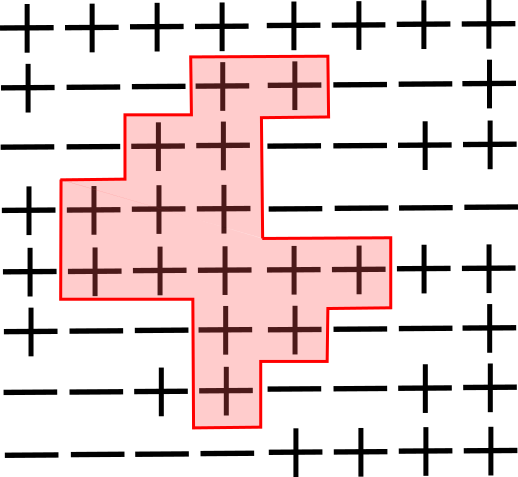
\includegraphics[scale=0.5]{esempioCluster.png}
\end{figure}

\end{center}
\end{frame}

\begin{frame}
\begin{center}
{\Large Swendsen and Wang algorithm:}

\begin{itemize}
\item Generate a link configuration $\sigma_{\langle x, y \rangle}$ based on the current spin configuration by using probablities $p_0$ and $p_1$. 
\item For each cluster chosse a spin $\left( s = \pm 1 \right)$ with probability $\frac{1}{2}$. In general the updte step must be compatible with the constraint $J_{\langle x, y \rangle}  s_x s_y = 1$ for all the spins of the cluster.
\item The newly generted spin configuration is the next element of the Markov chain.
\end{itemize}

\vspace{20pt}
The SW is \textbf{ergodic}. We know prove that it satisfy the \textbf{detailed balance}.

\end{center}
\end{frame}

\begin{frame}
\begin{center}
In the cluster algorithm we update both the spin $\lbrace s \rbrace$ and the links $\lbrace \sigma_{x, y} \rbrace$. The ensamble contains both spins and link configurations: $\lbrace s,  \sigma \rbrace$.

\[
\frac{P \left( \lbrace s_0, \sigma_0 \rbrace \rightarrow \lbrace s_1, \sigma \rbrace \right)}{ P \left( \lbrace s_1, \sigma_0 \rbrace \rightarrow \lbrace s_0, \sigma \rbrace \right)} = \frac{P \left( \lbrace s_1 \rbrace | \lbrace \sigma \rbrace \right) P \left( \lbrace \sigma \rbrace | \lbrace s_0 \rbrace \right) }{ P \left( \lbrace s_0 \rbrace | \lbrace \sigma \rbrace \right) P \left( \lbrace \sigma \rbrace | \lbrace s_1 \rbrace \right) }
\]

(this is not the detailer balance in the ensamble of $\lbrace s,  \sigma \rbrace$ as the lonk configurations don't get exchnged!)


\end{center}
\end{frame}


\begin{frame}
\begin{center}

$P \left( \lbrace s \rbrace | \lbrace \sigma \rbrace \right) =
 \frac{1}{2^{\# cluster}}$ if $\lbrace s \rbrace$ is compatible with $\lbrace \sigma \rbrace$, null otherwise.\\
\vspace{20pt} 
In general $P \left( \lbrace s \rbrace | \lbrace \sigma \rbrace \right)$ must be a \textbf{constant} independent of $\lbrace s \rbrace$ on the allowed configurations.\\
\vspace{20pt}
Thus $P \left( \lbrace s_1 \rbrace | \lbrace \sigma \rbrace \right) = P \left( \lbrace s_2 \rbrace | \lbrace \sigma \rbrace \right)$.

%In effetti questa probabilità non mi convince - rivedere.

%Dire che in realtà noi usiamo il sigle cluster algorithm con un procedimento ricorsivo (implementato con uno stack) che controlla una ed una sola volta ogni link per vedere se attivarlo o meno. Costruendo così un singolo cluster che andiamo a flippare.


\end{center}
\end{frame}

\begin{frame}
\begin{center}

{\large
\[P \left( \lbrace \sigma \rbrace | \lbrace s \rbrace \right) =
\prod_{ \substack{ \sigma_{\langle x, y \rangle} = 0 \\ J_{\langle x, y \rangle} s_x s_y = 1}} e^{-2 \beta} \prod_{\sigma_{\langle x, y \rangle} = 1} \left( 1- e^{-2 \beta } \right)
\]} for $\lbrace s \rbrace$ compatible with $\lbrace \sigma \rbrace$.\\
\vspace{20pt}
The first factor arise from the unconnected links for which $J_{\langle x, y \rangle} s_x s_y = 1$ each being in this state with probability $e^{ - 2 \beta }$. The second one is from the connected links (for which $J_{\langle x, y \rangle} s_x s_y = 1$ necessarily).\\
\vspace{20pt}
The second factor is \textbf{indipendent of $\lbrace s \rbrace$} and will be neglettend in the sequent.

\end{center}
\end{frame}

\begin{frame}
\begin{center}

We obtain:

\[
P \left( \lbrace \sigma \rbrace | \lbrace s \rbrace \right) =
\prod_{ \substack{ \sigma_{\langle x, y \rangle} = 0 \\ J_{\langle x, y \rangle} s_x s_y = 1}} e^{-2 \beta}
\]

Now we compute (reminding $\lbrace s_0 \rbrace$ and $\lbrace s_1 \rbrace$ share the same $\lbrace \sigma \rbrace$:

\begin{gather*}
\frac{e^{- \beta \mathcal{H} \left( \lbrace s_1 \rbrace \right)}}{e^{- \beta \mathcal{H} \left( \lbrace s_0 \rbrace \right)}} = \frac{\prod_{\langle x, y \rangle} e^{J_{\langle x, y \rangle} s^1_x s^1_y}}{\prod_{\langle x, y \rangle} e^{J_{\langle x, y \rangle} s^0_x s^0_y}} = \\ \frac{\prod_{\substack{\sigma = 0 \\ J s^1_x s^1_y = +1}} e^{\beta} \prod_{\substack{\sigma = 0 \\ J s^1_x s^1_y = -1}} e^{-\beta} \prod_{\substack{\sigma = 1 \\ J s^1_x s^1_y = +1}} e^{\beta}}{\prod_{\substack{\sigma = 0 \\ J s^0_x s^0_y = +1}} e^{\beta} \prod_{\substack{\sigma = 0 \\ J s^0_x s^0_y = -1}} e^{-\beta} \prod_{\substack{\sigma = 1 \\ J s^0_x s^0_y = +1}} e^{\beta}}
\end{gather*}

The last part having $\sigma = 1$ obviously depends only on $\lbrace \sigma \rbrace$ for all $J s_x s_y$ beeing forced to $1$ if $\sigma=1$.

\end{center}
\end{frame}

\begin{frame}
\begin{center}
We observe that: 
\[
\prod_{\substack{\sigma = 0 \\ J s^1_x s^1_y = -1}} e^{-\beta} \times \prod_{\substack{\sigma = 0 \\ J s^1_x s^1_y = 1}} e^{-\beta} = \prod_{\sigma = 0} e^{-\beta} = k
\] $k$ depends only on the link configuration $\lbrace \sigma \rbrace$\\

\[
\prod_{\substack{\sigma = 0 \\ J s^1_x s^1_y = -1}} e^{-\beta} = k \prod_{\substack{\sigma = 0 \\ J s^1_x s^1_y = 1}} e^{\beta} 
\]

\[
\frac{e^{- \beta \mathcal{H} \left( \lbrace s_1 \rbrace \right)}}{e^{- \beta \mathcal{H} \left( \lbrace s_0 \rbrace \right)}} = \frac{\prod_{\substack{\sigma = 0 \\ J s^1_x s^1_y = +1}} e^{2 \beta}} { \prod_{\substack{\sigma = 0 \\ J s^0_x s^0_y = +1}} e^{2 \beta}} = \frac{\prod_{\substack{\sigma = 0 \\ J s^0_x s^0_y = +1}} e^{-2 \beta}} { \prod_{\substack{\sigma = 0 \\ J s^1s_x s^0_y = +1}} e^{+2 \beta}}
\]

\end{center}
\end{frame}


\begin{frame}
\begin{center}

We arrived at:

\[
\frac{P \left( \lbrace s_0, \sigma_0 \rbrace \rightarrow \lbrace s_1, \sigma \rbrace \right)}{ P \left( \lbrace s_1, \sigma_0 \rbrace \rightarrow \lbrace s_0, \sigma \rbrace \right)} = \frac{e^{- \beta \mathcal{H} \left( \lbrace s_1 \rbrace \right)}}{e^{- \beta \mathcal{H} \left( \lbrace s_0 \rbrace \right)}}
\]

\[
P \left( \lbrace s_0 \rbrace \rightarrow \lbrace s_1\rbrace \right) = \sum_{\lbrace \sigma \rbrace, \lbrace \sigma_0 \rbrace} P \left( \lbrace s_0, \sigma_0 \rbrace \rightarrow \lbrace s_1, \sigma \rbrace \right)
\]

We thus obtain the detailed balance:

{ \Large
\[
\frac{P \left( \lbrace s_0 \rbrace \rightarrow \lbrace s_1\rbrace \right)}{P \left( \lbrace s_1 \rbrace \rightarrow \lbrace s_0\rbrace \right)} = \frac{e^{- \beta \mathcal{H} \left( \lbrace s_1 \rbrace \right)}}{e^{- \beta \mathcal{H} \left( \lbrace s_0 \rbrace \right)}}
\]
}

\end{center}
\end{frame}

\begin{frame}
\begin{center}

{\large
\begin{itemize}

\item The only requirement on the update step is that all the possible $\lbrace s \rbrace$ given $\lbrace s \rbrace$ which we choose to have a non null probability of happearing are indeed equiprobable.
\item We can also update the coupling constants $J_{\langle x, y \rangle}$ as long as $J_{\langle x, y \rangle}$ where $\sigma = 1$.

\end{itemize}}

This two observations give rise to two key modification of the SW algorithm: the Wolff algorithm and the boundary flip.

\end{center}
\end{frame}

\begin{frame}
\begin{center}
{
\Large Single cluster update:\\
}
\vspace{10pt}
In the Wolff algorithm we chose at random one site of the lattice and flipping the cluster it belongs to with certanty.\\
\vspace{10pt}
It is equivalent to chossing at random one site of the lattice and consider it the seed for and expanding cluster and then flipping it.  

\begin{figure}[!htb]
\centering
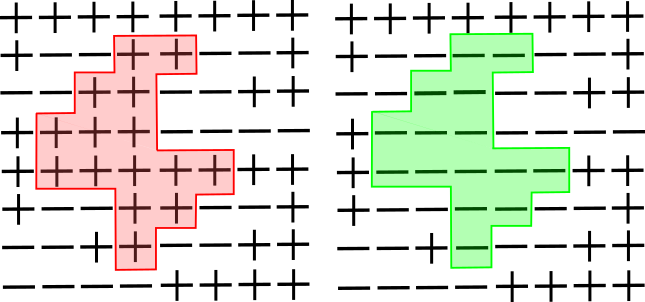
\includegraphics[scale=0.4]{wolff.png}
\end{figure}

%TODO--Questa cosa non mi torna: "we chose at random one site of the lattice" or "we chose at random a cluster".

\end{center}
\end{frame}

\begin{frame}
\begin{center}

{\Large Boundary flip algorithm:\\}
\vspace{20pt}
$J = 1$ in the bulk, but the coupling between the top and the bottom is now a dynamical variable to simulate: $\lbrace s, \sigma, J_{0, T-1} = \pm 1 \rbrace$.\\
\vspace{20pt}
A link $\sigma_{\langle 0, T-1 \rangle} = 1$ demands $J_{0, T-1} s_0 s_{T-1} = 1$. Thus we can flip $J_{0, T-1}$, $s_0$ and all the spins connected to $s_0$ via some chain of links in the bulk obtaing a configuration compatible with $\lbrace \sigma_{\langle x, y \rangle} \rbrace $. This for all the spins on the bottom boundary.

\end{center}
\end{frame}

\begin{frame}
\begin{center}
\begin{columns}
\begin{column}{0.20\textwidth}
\begin{center}
Boundary condition update.
Section of a $7 \times 7 \times 21$ lattice at temperature $\beta = 0.250$
\end{center}
\end{column}
\begin{column}{0.80\textwidth}
\begin{figure}[!htb]
\centering
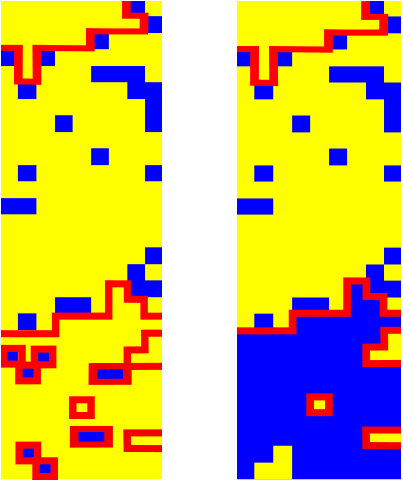
\includegraphics[scale=0.5]{boundaryFlip.png}
\end{figure}

\end{column}
\end{columns}

\end{center}
\end{frame}

\begin{frame}
\begin{center}
{ \large The boundary flip generates an interface between phases!\\ } 
\vspace{20pt}
We must check this update can be done without violating the constraints imposed by the bulk links ($\sigma_{\langle x, y \rangle} = 1$ implies $s_x = s_y$).\\
\vspace{20pt}
Check all the clusters that contain sites of the lower surface and flip the boundary condition only if it can be done consistently on all the lattice.
\end{center}
\end{frame}

\begin{frame}
\begin{center}

\begin{columns}
\begin{column}{0.30\textwidth}
\begin{center}
Introduce an extra variable $c_{x} = \pm 1$ that gets propagated in the bulk during the costruction of the cluster but changes sign when crossing the boundary.
\end{center}
\end{column}
\begin{column}{0.70\textwidth}

\begin{figure}[!htb]
\centering
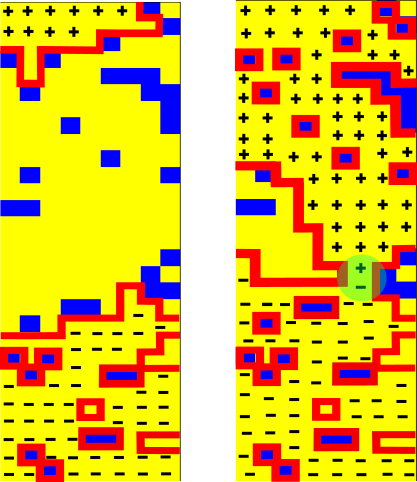
\includegraphics[scale=0.5]{extra.png}
\end{figure}

\end{column}
\end{columns}

\end{center}
\end{frame}

\begin{frame}
\begin{center}
%The boundary flip is ergodic
We do $N$ total steps alternating the Wolff algorithm with the boundary flip.\\
\vspace{20pt}
After each update we count if the current configuration has ferromagnetic or antiferromagnetic coupling between top and bottom.\\ 
\[
\langle \delta_{J = -1} \rangle = \frac{\# \text{Antiferromagnetic}}{N}
\]
\[
\langle \delta_{J = +1} \rangle = \frac{\# \text{Ferromagnetic}}{N}
\]

\end{center}
\end{frame}


\begin{frame}{Notes on the implementation}
\begin{center}

C++ for the Montecarlo and Jackknife algorithms, Python for data analysis, fits and plots.\\
\vspace{20pt}
The hot function of the simulation generates a cluster starting in a given position and exploring the neighbouring links. If a link is chosen to be $\sigma_{\langle x, y \rangle} = 1$ then the adjacent site is included in the cluster and the procedure is repeated. The extra variable $c_x$ is also propagated.
\end{center}
\end{frame}


\begin{frame}

stack<site> stack

stack.push(seed)

while(!stack.empty())

\quad site current = stack.top()

\quad value = cluster[current]

\quad if(cluster[current] is incostintent) flag = 1;

\quad else if(cluster[current] == 0)

\quad \quad cluster[current] = cluster[old];

\quad \quad for(d = 0; d < 3; d++) 

\quad \quad \quad for(a = -1; a < 2; a = a + 2) 

\quad \quad \quad next = current + a

\quad \quad \quad Check if we are on the boundary
				
\quad \quad \quad if(cluster[next] == 0)

\quad \quad \quad \quad if(p > 0 and random < p) stack.push(next)\\
return flag

\end{frame}


\begin{frame}
\begin{center}
\begin{itemize}
\item The algorithm doesn't actually performs the spin and boundary flip it just counts for how many configuration it is possible.\\
\vspace{10pt}
\item The simulation where executed with $N = 10^5, 10^6$ steps of the Markov chain.\\
\vspace{10pt}
\item The first $5\%$ of the Markov chain is ignored to avoid non-termalized configurations.\\
\vspace{10pt}
\item The Jackknife is executed for blocks with size starting from $10000$ to $10900$ with step of $30$ events. 
\end{itemize}
\end{center}
\end{frame}

\begin{frame}{Estimation of the errors and autocorrelation}
\begin{center}

\end{center}
\end{frame}

\begin{frame}{Fit of the free energy - theory}
\begin{center}

\end{center}
\end{frame}

\begin{frame}{Fit of the free energy - results}
\begin{center}

\end{center}
\end{frame}

\begin{frame}{Fit of the critical behaviour}
\begin{center}

\end{center}
\end{frame}

\begin{frame}{(Conclusions?)}
\begin{center}

\end{center}
\end{frame}

%----------------------------------------------------------------------------------------

\end{document} 